\documentclass[a4paper]{article}
\usepackage[utf8]{inputenc}   % pro unicode UTF-8
\usepackage[czech]{babel} %jazyk dokumentu
\usepackage{listings}
\usepackage{color}
\usepackage[T1]{fontenc}
\usepackage{amssymb}
\usepackage{hyperref}
\usepackage{listingsutf8}
\usepackage{graphicx}
\usepackage{amsmath}
\usepackage{multicol}
\usepackage[margin={1cm,2cm}]{geometry}

\graphicspath{ {/} }

\setcounter{MaxMatrixCols}{40}
\def\doubleunderline#1{\underline{\underline{#1}}}

%%%%%%%%%%%%%%%%%%%%%%%%%%%%%%%%%%%%%%%%%%%%%%%%%%%%%%%%%%%%%

\begin{document}

\noindent
\textbf{Predmet: Kombinatorika a grafy 1}\\
\textbf{Ukol: 2.}\\
\textbf{Verze: 1.}\\
\textbf{Autor: David Napravnik}

\section*{Prvni ukol}
\subsection*{$a_0 = 2, a_1=3, a_{n+2} = 3a_n-2a_{n+1}$}

\begin{tabular}{ c c c c c c }
	A(0) & A(1) & A(2) & A(3) & & A(x)\\ 
	2 & 3 & 3A(0)-2A(1) & 3A(1)-2A(2) & & ||\\ 
	\hline
	2 & 7 & 0 & 0 & \dots & $2+7x$\\ 
	0 & -2A(0) & -2A(1) & -2A(2) & \dots & $-2xA(x)$\\ 
	0 & 0 & 3A(0) & 3A(1) & \dots & $3x^2A(x)$\\
\end{tabular}
\noindent
$A(x)2+7x-2xA(x)+3x^2A(x)\\
A(x)+2xA(x)-3x^2A(x) = 7x+2\\
A(x)(1+2x-3x^2) = 7x+2\\
A(x) = \frac{7x+2}{1+2x-3x^2} = \frac{1}{4}\left(\frac{-1}{1-(-3x)}+\frac{9}{1-x}\right)\\
A(x) = \frac{9-(-3)^x}{4}
$


\subsection*{$a_0 = 0, a_1=1, a_{n+2} = a_{n+1} + 2a_n + 2$}

\begin{tabular}{ c c c c c c }
	A(0) & A(1) & A(2) & A(3) & & A(x)\\ 
	0 & 1 & 2+2A(1)+A(0) & 2+2A(2)+A(1) & & ||\\ 
	\hline
	0 & 1 & 0 & 0 & \dots & $x$\\ 
	0 & 0 & 2 & 2 & \dots & $2x^2$\\ 
	0 & A(0) & A(1) & A(2) & \dots & $xA(x)$\\ 
	0 & 0 & 2A(0) & 2A(1) & \dots & $2x^2A(x)$\\
\end{tabular}
\noindent
$
A(x)= x+2x^2+x A(x)+2x^2A(x)\\
A(x)(1-x-2x^2) = x+2x^2\\
A(x) = \frac{x+2x^2}{1-x-2x^2}\\
A(x) = \frac{-2}{3(2x-1)}+\frac{1}{3(x+1)}-1\\
A(x) = 2^x-1\\
$




\section*{Druhy ukol}
Pro $x = 1$ je pocet vydlazdeni roven $1$.\\
Pro $x = 2$ je pocet vydlazdeni roven $2$ (svisle, nebo horizontalne).\\
Pro $x > 2$ je pocet vydlazdeni roven $F_{x-1}$ (x-prvni Fibonaciho cislo).\\\\
Protoze: mejme jiz nejak vydlazdeny chodnik delky $x-1$, a chceme jej prodlouzit
o jednu cihlu. To muzeme udelat tak, ze ji pridame za cely chodnik a
takovych vydlazdeni je prave stejne jako pocet vydlazdeni u $x-1$ dlouheho chodniku,
nebo jednu cihlu odebereme a pridame dve nove tak,
ze novy usek chodniku je pokryt dvemi polovinami cihlicek.
Takovych variant pokryti je jako u $x-2$ dlouheho chodniku.\\
Proto stejne jako u fibonaciho cisla: $F_x = F_{x-1} + F_{x-2}$

\section*{Treti ukol}
\subsection*{not A1}
$X = \{a,b,c,d\}$\\
$P = \{P_1, P_2, P_3\} = \{\{a,b\},\{b,c\},\{a,c\}\}$\\
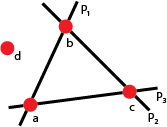
\includegraphics[width=100px]{hw2-1.png}

\subsection*{non A2}
$X = \{\{a,b,c,d\}\}$\\
$P = \{P_1, P_2, P_3, P_4\} = \{\{c,d\},\{a,c\},\{b,c\},\{b,d\},\{\}\}$\\
\includegraphics[width=100px]{hw2-2.png}


\section*{Ctvrty ukol}
Mejme 1 bod, z nej podle definice musi vychazet $n+1$ primek.
A na kazde primce je dalsich $n$ bodu pricemz jsou tyto bod rozdilne.
tudiz mame $n(n+1)$ bodu plus ten jeden, ze ktereho jsme vychazeli.




\end{document}